\documentclass[../../main.tex]{subfiles}
\begin{document}

{\bf [解答]}

\paragraph{(1)}

\begin{figure}[htb]
  \centering
  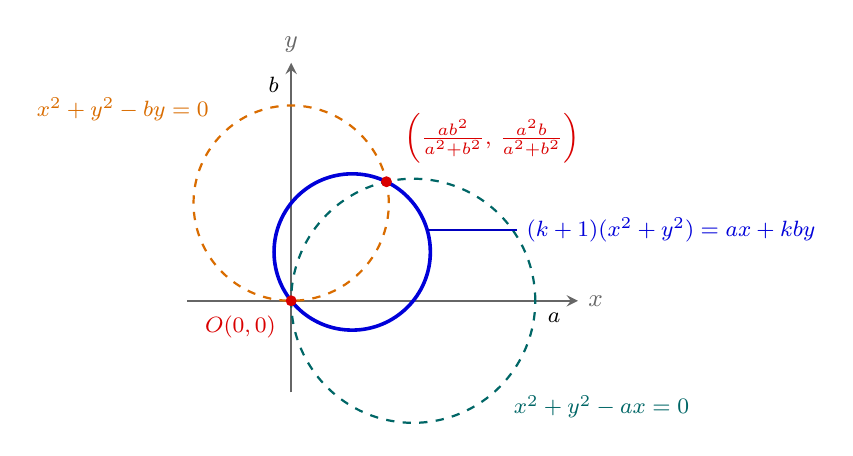
\begin{tikzpicture}[x=1.55cm, y=1.55cm, >=stealth, every node/.style={font=\small}]
    % 図示用パラメータ: a=2.0, b=1.6, k=1.0
    % 円1: (x-1)^2 + y^2 = 1, 円2: x^2 + (y-0.8)^2 = 0.64
    % 題意の円 (k=1): (x-0.5)^2 + (y-0.4)^2 = 0.41
    % 交点: O(0,0), P(ab^2/(a^2+b^2), a^2b/(a^2+b^2)) = (128/164, 160/164) ≈ (0.7805, 0.9756)
    \coordinate (O) at (0, 0);
    \coordinate (P) at (0.7805, 0.9756);

    \draw[->, thick, gray!80!black] (-0.85, 0) -- (2.35, 0) node[right] {$x$};
    \draw[->, thick, gray!80!black] (0, -0.75) -- (0, 1.95) node[above] {$y$};

    % 2つの基準円
    \draw[thick, dashed, teal!80!black] (1.0, 0) circle (1.0);
    \draw[thick, dashed, orange!85!black] (0, 0.8) circle (0.8);

    % 題意の円 (k=1)
    \draw[line width=1.3pt, blue!85!black] (0.5, 0.4) circle ({sqrt(0.41)});

    % ラベル
    \node[teal!80!black, font=\footnotesize, below right=2pt] at (1.7, -0.65) {$x^2+y^2-ax=0$};
    \node[orange!85!black, font=\footnotesize, above left=2pt] at (-0.55, 1.35) {$x^2+y^2-by=0$};
    \draw[thin, blue!75!black] (1.11, 0.58) -- (1.85, 0.58)
    node[right, font=\footnotesize, blue!85!black] {$(k+1)(x^2+y^2)=ax+kby$};

    \node[below right=1pt, font=\footnotesize] at (2.0, 0) {$a$};
    \node[above left=1pt, font=\footnotesize] at (0, 1.6) {$b$};

    % 2定点
    \node[circle, fill=red!85!black, inner sep=1.4pt] at (O) {};
    \node[below left=2pt, font=\footnotesize, red!85!black] at (O) {$O(0,0)$};
    \node[circle, fill=red!85!black, inner sep=1.4pt] at (P) {};
    \node[above right=3pt, font=\footnotesize, red!85!black] at (P)
    {$\left(\frac{ab^2}{a^2+b^2},\,\frac{a^2b}{a^2+b^2}\right)$};
  \end{tikzpicture}
  \caption{2円 $x^2+y^2-ax=0$, $x^2+y^2-by=0$ とその交点を通る円}
  \label{fig:1962_2_circles}
\end{figure}

円の方程式
\begin{align}
  (k+1)(x^2+y^2) = ax + kby \label{eq:1}
\end{align}
を$k$について整理すると
\begin{align}
  k(x^2 + y^2 - by) + (x^2 + y^2 - ax) = 0
\end{align}
だから，これが$k\neq -1$なる任意の$k$で成り立つには
\begin{align}
  \begin{cases}
    x^2 + y^2 - by = 0 \\
    x^2 + y^2 - ax = 0
  \end{cases}
\end{align}
である．これを解くと
\begin{align}
  (x, y) = (0, 0), \left( \dfrac{ab^2}{a^2+b^2}, \dfrac{a^2 b}{a^2+b^2} \right)
\end{align}
だから，題意の円はこの二点を通る．

\paragraph{(2)}

円の中心 $M(X, Y)$ とすると\cref{eq:1}より
\begin{align}
  X = \dfrac{a}{2(k+1)}, \quad Y = \dfrac{kb}{2(k+1)} \label{eq:2}
\end{align}
である．題意より$a \ne 0$ から $X \ne 0$ だから，$\dfrac{Y}{X}$を計算すると
\begin{align}
  \dfrac{Y}{X} = \dfrac{b}{a} k
  \quad \therefore
  k = \dfrac{a}{b} \dfrac{Y}{X} \quad (\because b \ne 0)
\end{align}
である．これを\cref{eq:2}に代入して
\begin{align}
  X = \dfrac{a}{2\left( \dfrac{a}{b} \dfrac{Y}{X} + 1 \right)} = \dfrac{abX}{2(aY + bX)}
\end{align}
である．
$X \ne 0$ で両辺を割って
\begin{align}
  2(aY + bX) = ab \quad (X \ne 0)
\end{align}
である．よって軌跡の方程式は
\begin{align}
  2bx + 2ay = ab \quad (x \ne 0)
\end{align}
となる．

{\bf [解説]}

\begin{figure}[htb]
  \centering
  \begin{tikzpicture}[x=1.8cm, y=1.8cm, >=stealth, every node/.style={font=\small}]
    % a=2.0, b=1.6 => A(0,0), B(0.7805, 0.9756), 中点 N(0.3902, 0.4878)
    % 垂直二等分線: 2bx + 2ay = ab <=> 3.2x + 4.0y = 3.2 <=> y = 0.8 - 0.8x
    \coordinate (A) at (0, 0);
    \coordinate (B) at (0.7805, 0.9756);
    \coordinate (N) at (0.3902, 0.4878);
    \coordinate (M) at (0.65, 0.28);

    \draw[->, thick, gray!80!black] (-0.55, 0) -- (1.95, 0) node[right] {$x$};
    \draw[->, thick, gray!80!black] (0, -0.45) -- (0, 1.55) node[above] {$y$};

    % 定点 A, B を通る円の例（中心 M）
    \draw[dashed, teal!75!black] (M) circle ({sqrt(0.65^2 + 0.28^2)});
    \draw[dashed, gray!70!black] (A) -- (M) -- (B);

    % 弦 AB
    \draw[thick, blue!85!black] (A) -- (B);

    % 中心の軌跡（線分 AB の垂直二等分線，x=0 を除く）
    \draw[line width=1.3pt, red!80!black] (-0.35, 1.08) -- (1.55, -0.44)
    node[below right=1pt, font=\footnotesize] {$2bx+2ay=ab$};

    % 直角記号
    \draw[gray!80!black] ($(N)!0.11cm!(B)$)
    -- ($($(N)!0.11cm!(B)$)!0.11cm!90:(B)$)
    -- ($(N)!0.11cm!90:(B)$);

    % 点とラベル
    \node[circle, fill=blue!85!black, inner sep=1.4pt] at (A) {};
    \node[below left=2pt, font=\footnotesize, blue!85!black] at (A) {$A(0,0)$};
    \node[circle, fill=blue!85!black, inner sep=1.4pt] at (B) {};
    \node[above right=2pt, font=\footnotesize, blue!85!black] at (B)
    {$B\left(\frac{ab^2}{a^2+b^2},\,\frac{a^2b}{a^2+b^2}\right)$};

    \node[circle, fill=teal!85!black, inner sep=1.3pt] at (M) {};
    \node[above right=2pt, font=\footnotesize, teal!85!black] at (M) {$M(X,Y)$};

    % x=0 の除外点 (0, b/2)
    \node[circle, draw=red!80!black, thick, fill=white, inner sep=1.4pt] at (0, 0.8) {};
    \node[left=3pt, font=\footnotesize] at (0, 0.8) {$\frac{b}{2}$};
    \node[below=2pt, font=\footnotesize] at (1.0, 0) {$\frac{a}{2}$};
  \end{tikzpicture}
  \caption{2定点 $A,B$ を通る円の中心 $M$ の軌跡（線分 $AB$ の垂直二等分線）}
  \label{fig:1962_2_perp_bisector}
\end{figure}

(2)で求めた直線は，(1)で求めた定点を$A,B$として線分$AB$の垂直二等分線になっているはずである．
これは検算として使える．実際にやってみよう．

$AB$の垂直二等分線の方程式は
\begin{align}
  & y = -\dfrac{b}{a} \left( x - \dfrac{ab^2}{2(a^2+b^2)} \right) + \dfrac{a^2 b}{2(a^2+b^2)} \\
  & y = -\dfrac{b}{a} x + \dfrac{b(a^2+b^2)}{2(a^2+b^2)} \\
  & bx + ay = \dfrac{1}{2} ab  \\
\end{align}
となり，確かに(2)で求めた方程式と一致する．

\newpage

\end{document}
